\documentclass{article}
\usepackage{qilin}
\tikzstyle{process} = [rectangle, rounded corners, minimum width=1.5cm, minimum height=0.5cm,align=center, draw=black, fill=gray!30, auto]
\title{MAT257: Real Analysis II}
\author{QiLin Xue}
\date{Fall 2021}
\usepackage{mathrsfs}
\usetikzlibrary{arrows}
\usepackage{stmaryrd}

\begin{document}

\maketitle
\tableofcontents
\newpage
\section{Differentiation}
\subsection{Inverse Function Theorem}
\begin{theorem}
    Suppose that $f:\mathbb{R}^n \rightarrow \mathbb{R}^n$ is continuously differentiable in an open set containing $a$ and $\det f'(a) \neq 0$. Then there is an open set $V$ containing $a$ and an open set $W$ containing $f(a)$ such that $f:V\rightarrow W$ has a continuous inverse $f^{-1}:W\rightarrow V$ which is differentiable and for all $y\in W$ satisfies
    \begin{equation}
        (f^{-1})'(y) = [f'(f^{-1}(y))]^{-1}
    \end{equation}
\end{theorem}
\textit{Motivation:} In 1D calculus, if a function has a derivative $f'(x)>0$ at some point $x=a$, then around this point the function is monotone and has an inverse, per the intermediate value theorem. We want something similar for multiple dimensions, however there is no equivalent intermediate value theorem.

We will motivate our proof with the following steps
\begin{enumerate}
    \item Prove the last step, as it is the easiest.
    \item WLOG, make the simplifying assumption that $f'(a) = I$.
    \item Define ``all-scale fidelity'' to describe how vectors in an open neighbourhood around $a$ are \textit{nearly} preserved.
\end{enumerate}
Let us perform these steps:
\begin{enumerate}
    \item Consider the following setup
    \begin{center}
        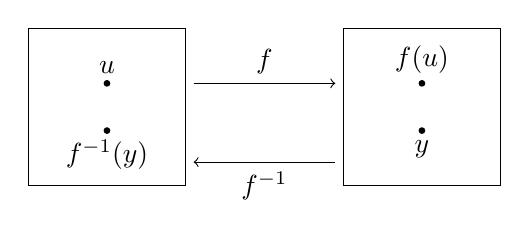
\begin{tikzpicture}
            
            \draw[] (0,0) rectangle (2,2);
            \draw[->] (2.1, 1.3) -- (3.9, 1.3) node[above, midway] {$f$}; 
            \draw[<-] (2.1, 0.3) -- (3.9, 0.3) node[below, midway] {$f^{-1}$}; 

            \draw[] (4,0) rectangle (6,2);

            
            \filldraw[black] (1,1.3) circle (1pt) node[anchor=south]{$u$};
            \filldraw[black] (5,1.3) circle (1pt) node[anchor=south]{$f(u)$};
            \filldraw[black] (1,0.7) circle (1pt) node[anchor=north]{$f^{-1}(y)$};
            \filldraw[black] (5,0.7) circle (1pt) node[anchor=north]{$y$};

        \end{tikzpicture}
    \end{center}
    Recall that $f \circ f^{-1} = I$, so differentiating and applying the chain rule we can write 
    \begin{equation}
        f'(f^{-1}(y)) \cdot (f^{-1})'(y) = I \implies (f^{-1})'(y) = [f'(f^{-1}(y))]^{-1}
    \end{equation}
    \item We are allowed to write $f'(a) = I$ since every invertible matrix is just the identity with a change of basis. More concretely, consider another composition represented below, where $L=f'(a):$
    \begin{center}
        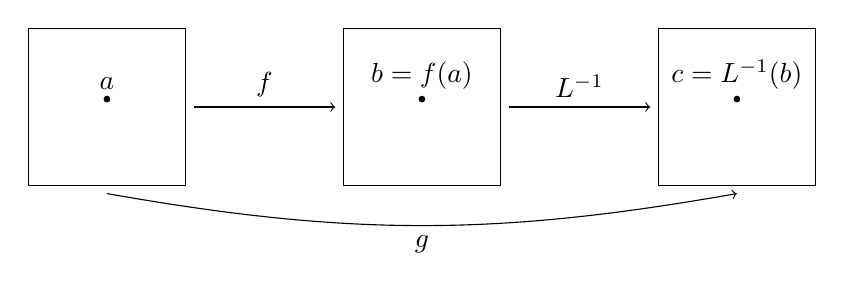
\begin{tikzpicture}
            
            \draw[] (0,0) rectangle (2,2);
            \draw[->] (2.1, 1) -- (3.9, 1) node[above, midway] {$f$}; 
            \draw[->] (6.1, 1) -- (7.9, 1) node[above, midway] {$L^{-1}$}; 

            \draw[] (4,0) rectangle (6,2);
            \draw[] (8,0) rectangle (10,2);

            
            \filldraw[black] (1,1.1) circle (1pt) node[anchor=south]{$a$};
            \filldraw[black] (5,1.1) circle (1pt) node[anchor=south]{$b=f(a)$};
            \filldraw[black] (9,1.1) circle (1pt) node[anchor=south]{$c=L^{-1}(b)$};

            \draw [->,black] (1,-0.1) to [out=-10,in=190] node[below, midway] {$g$} (9,-0.1);

        \end{tikzpicture}
    \end{center}
    By the chain rule, we have $g'(a) = L^{-1} \circ f'(a)$ since $L^{-1}$ is a linear transformation. Note that $f'(a) = L$, so $g'(a) = I$ is the identity.

    If the IFT was true for functions whose differential is $I$, then it's true for $g$, so there exists $g^{-1}$. Also, $f^{-1} = g^{-1} \circ L^{-1}.$ Therefore, if $g^{-1}$ is continuously differentiable, then $f^{-1}$ would also be continuously differentiable. Thus, it is sufficient to only look at the case where the differential is the identity.
\end{enumerate}
\end{document}